\documentclass{amsart}

%%%%%%%%%%%%%%%

\usepackage[utf8]{inputenc}
% \usepackage[spanish]{babel}
% \usepackage[top=1in, bottom=1in, left=1.2in, right=1.2in]{geometry}
\usepackage{amssymb}
\usepackage{amsmath}
\usepackage{amsfonts}
\usepackage{amsthm}
\usepackage{wasysym}
\usepackage{enumitem}
\usepackage{graphicx}
\usepackage{listings}
\usepackage{xcolor}
\usepackage{tikz}

% sets
\newcommand{\NN}{\mathbf{N}}
\newcommand{\ZZ}{\mathbf{Z}}
\newcommand{\QQ}{\mathbf{Q}}
\newcommand{\RR}{\mathbf{R}}
\newcommand{\Zpos}{\ZZ^{+}}
\newcommand{\Rpos}{\RR^{+}}

% brackets
\newcommand{\la}{\langle}
\newcommand{\ra}{\rangle}

% formal statements
\newtheorem{prop}{Proposition}

\theoremstyle{plain}
\newtheorem{clm}{Claim}

\theoremstyle{definition}
\newtheorem{defn}{Definition}

\newtheorem{exl}{Example}

\theoremstyle{remark}
\newtheorem{rmk}{Remark}

% vulgar display of code

\lstdefinestyle{astyle}{
	commentstyle=\color{blue},
	keywordstyle=\color{purple},
	numberstyle=\tiny\color{gray},
	stringstyle=\color{green},
	basicstyle=\ttfamily\footnotesize,
	tabsize=2
}

\lstset{style=astyle}


\title{Work log of June 17}
\author{Daniel R. Barrero R.}
\date{\today}

\begin{document}

\maketitle

\section{}

The operad-given monad according to Milewski seems to be defined as

\lstinputlisting[language=Haskell, firstline=39]{DocCode.hs}

Which is confusing to me since it doesn't resemble May's very much. However, it's
arguably easy to picture it, since one expects the coefficients of the vector to become
the tree's leaves.

\bigskip
\bigskip

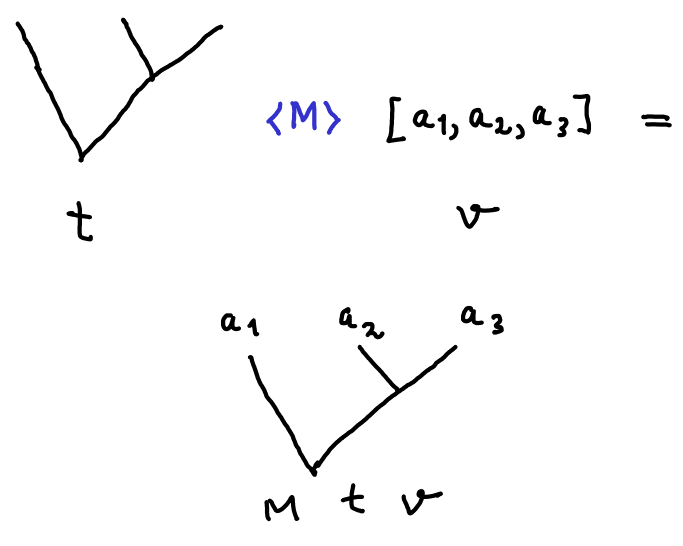
\includegraphics[width=0.5\textwidth]{tree_w_vecComp}

\section{Comments}

\begin{itemize}
	\item A tree whose leaves are \texttt{a-}type-trees can be put together into a
		big \texttt{a-}type-tree in the obvious way.
\end{itemize}
\end{document}
